\section{Contexto y Motivaci�n}

\subsection{Memoria Corporativa}
\begin{frame}
	\frametitle{Memoria Corporativa}
	%%%%%%%%%%%%%%%%%%%%%%%
	\begin{block}{Definici�n}
	\justifying 
	La representaci�n expl�cita, t�cita, consistente y persistente del conocimiento de una organizaci�n. \cite{Ontoinra2002}
	\end{block}
	
	\begin{figure}[htbp]
	\centering
	\subfigure{
	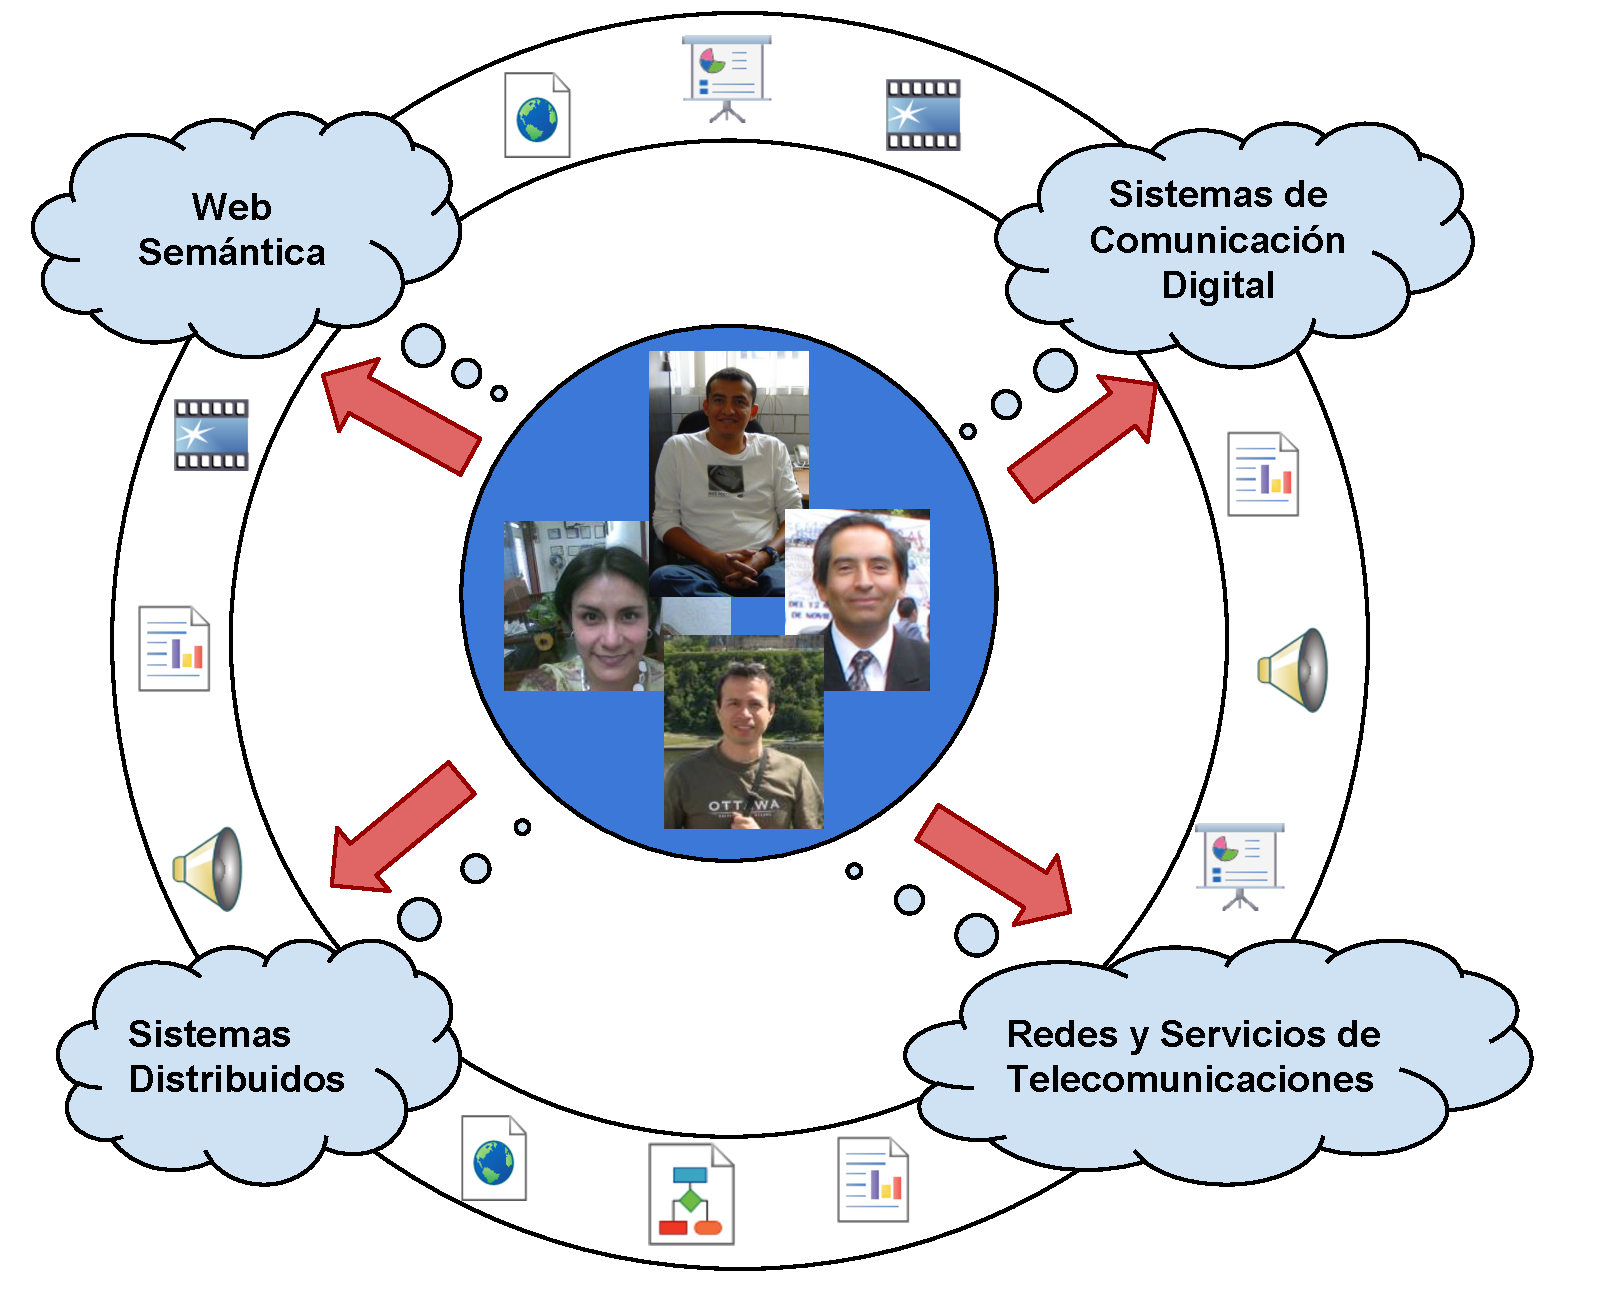
\includegraphics[scale=0.18]{ConocimientoRyT} 
	}
	\subfigure{
	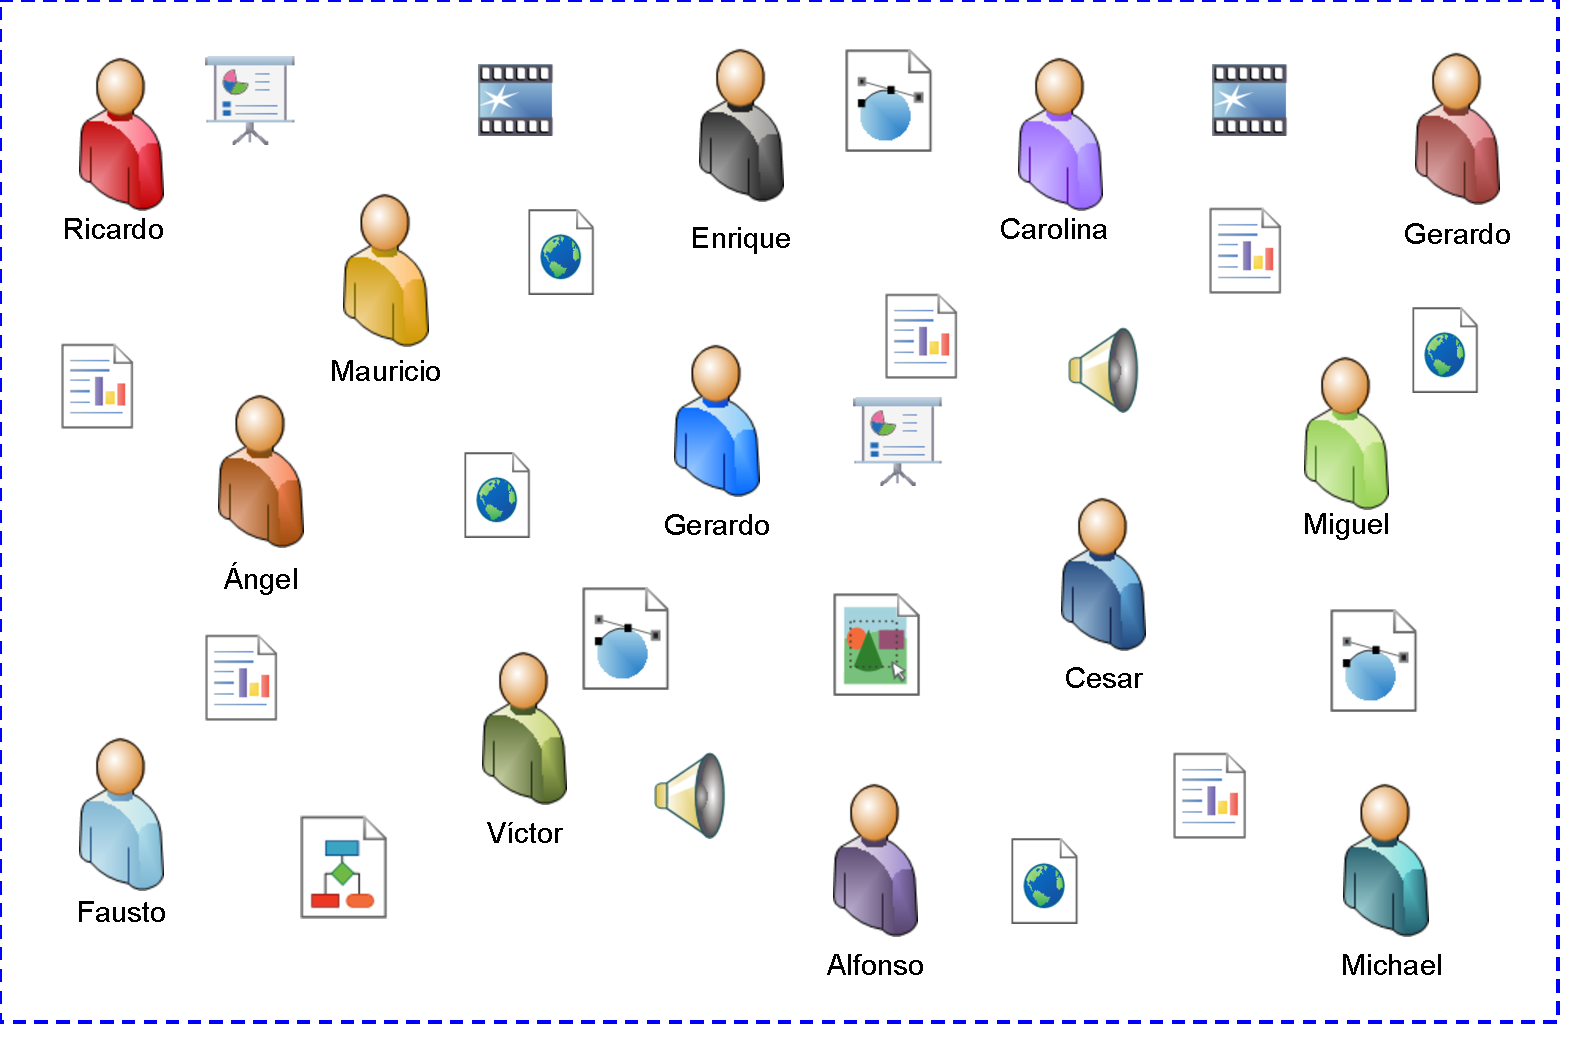
\includegraphics[scale=0.19]{EjemploMC} 
	}
	\end{figure}
	%%%%%%%%%%%%%%%%%%%%%%%
\end{frame}

\subsection{Integraci�n Sem�ntica}
\begin{frame}
	\frametitle{Integraci�n Sem�ntica}
	\begin{block}{Definici�n}
	\justifying
	La b�squeda y recuperaci�n significativa de informaci�n existente en los recursos de informaci�n para responder una consulta dada por un usuario.
	\end{block}
	
	\begin{exampleblock}{Etapas}
	\begin{enumerate}[<+-| alert@+>]
	\item \justifying Construir un modelo para representar el conocimiento de los \textit{recursos de informaci�n} existentes en una \textit{memoria corporativa}.
	\item \justifying Buscar y recuperar informaci�n existente en la memoria corporativa, mediante la interrogaci�n del modelo.
	\end{enumerate}
	\end{exampleblock}
\end{frame}

\begin{frame}
	\frametitle{Heterogeneidad y Significado de la Informaci�n}
	\begin{figure}
	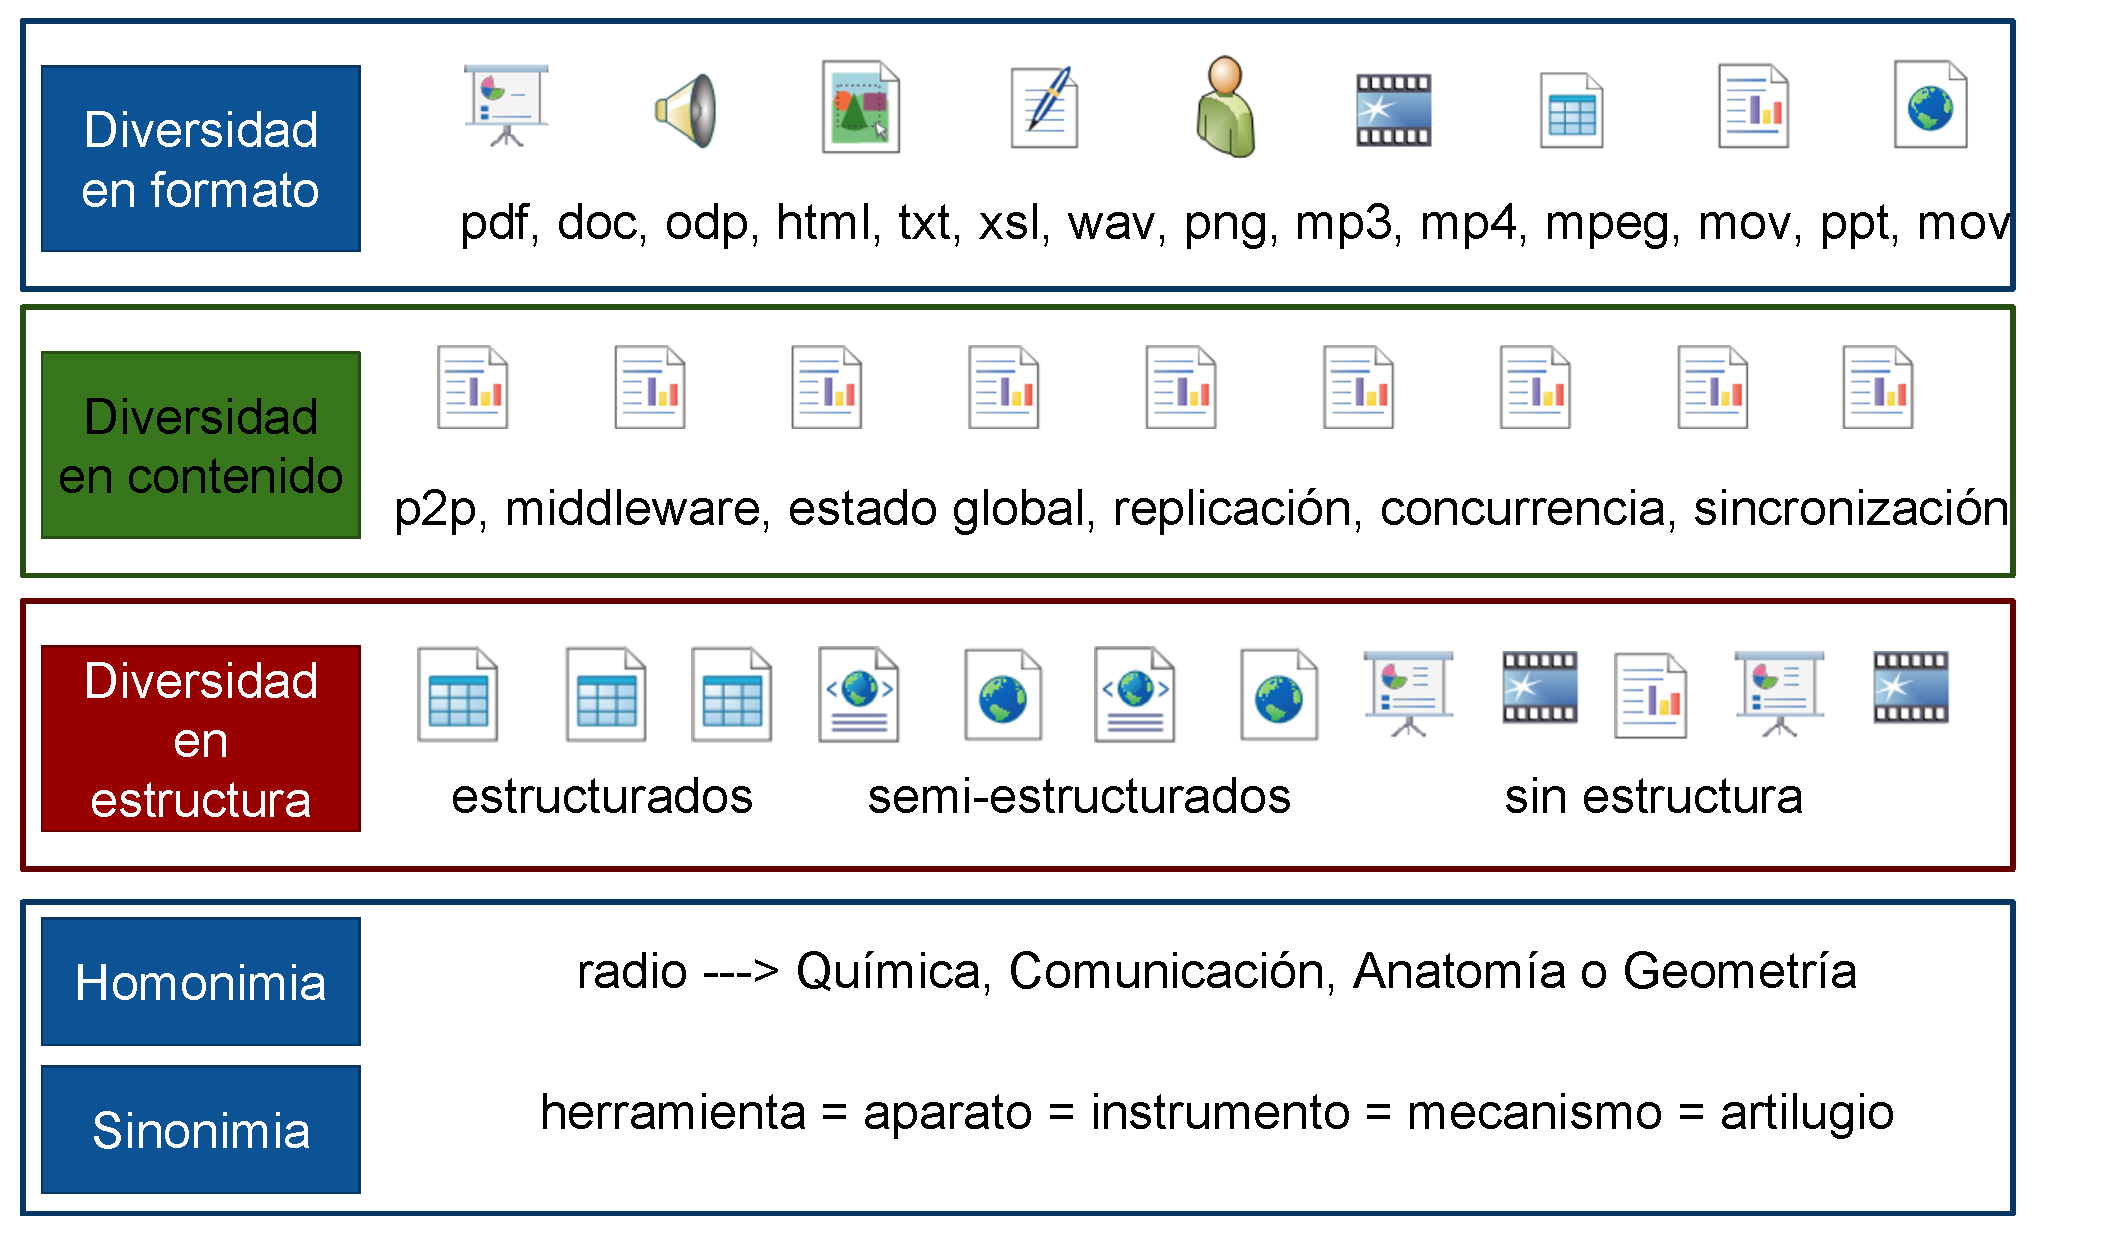
\includegraphics[scale=0.30]{NatMC} 
	\end{figure}
\end{frame}

\subsection{Tecnolog�as Sem�nticas}
\begin{frame}
	\frametitle{Tecnolog�as Sem�nticas}
	\begin{block}{Definici�n}
	\justifying 
	\textit{Un conjunto de metodolog�as, lenguajes, aplicaciones, herramientas y est�ndares para suministrar u obtener el significado de las palabras, informaci�n y las relaciones entre �stos}. \begin{scriptsize}\cite{SemTecRetr}\end{scriptsize}
	\end{block}
	
	\begin{figure}
	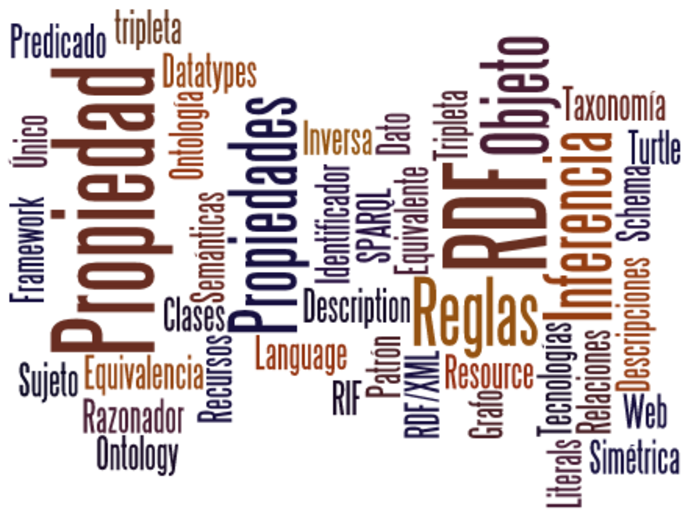
\includegraphics[scale=0.42]{TSWords} 
	\end{figure}
\end{frame}

\begin{frame}
	\frametitle{Tecnolog�as Sem�nticas}
	%%%%%%%%%%%%%%%%%%%%%%%%%%%%
	\begin{alertblock}{Ontolog�a}
	\justifying 
	Una definici�n formal, expl�cita y compartida de los conceptos, as� como las relaciones de un determinado dominio. \begin{scriptsize}\cite{Gruber}\end{scriptsize}
	\end{alertblock}
	
%	\begin{block}{Componentes}
%	\begin{itemize}
%	\item \justifying Componente Asertivo (ABox) est� constituido por descripciones que afirman que los individuos son instancias de una clase o propiedad.
%	\item \justifying Componente Terminol�gico (TBox) describe las clases y propiedades relevantes, as� como las reglas de inferencia que permiten aprovechar la manera en que las instancias se relacionan entre s�.
%	\end{itemize}
%	\end{block}
	
	\begin{figure}
	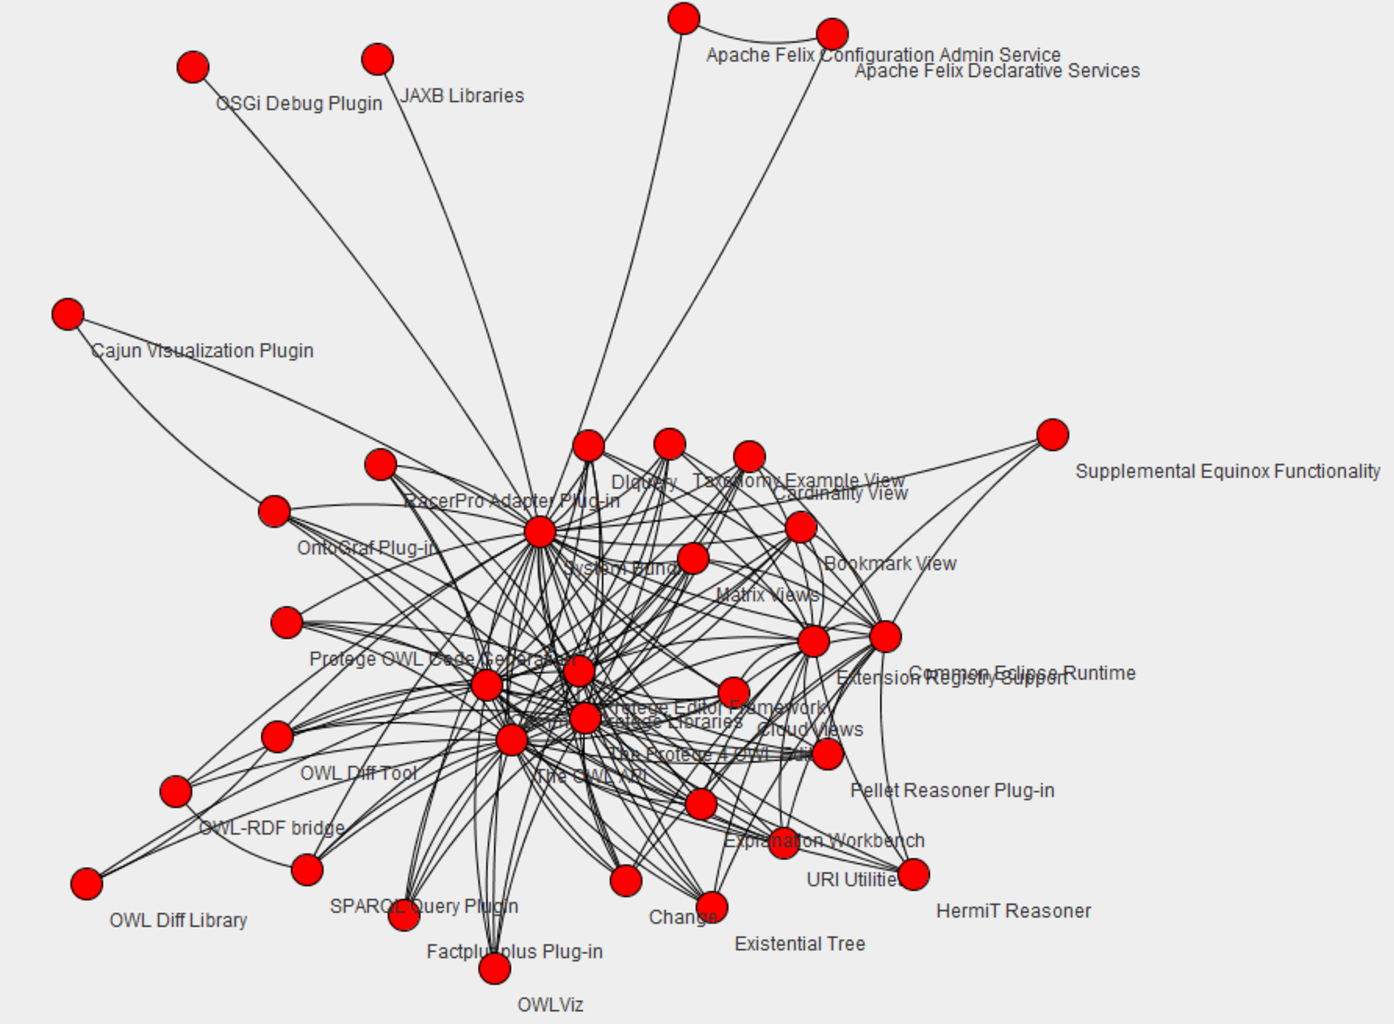
\includegraphics[scale=0.25]{OntoGraph} 
	\end{figure}
\end{frame}